\documentclass[]{article}
\usepackage{lmodern}
\usepackage{amssymb,amsmath}
\usepackage{ifxetex,ifluatex}
\usepackage{fixltx2e} % provides \textsubscript
\ifnum 0\ifxetex 1\fi\ifluatex 1\fi=0 % if pdftex
  \usepackage[T1]{fontenc}
  \usepackage[utf8]{inputenc}
\else % if luatex or xelatex
  \ifxetex
    \usepackage{mathspec}
  \else
    \usepackage{fontspec}
  \fi
  \defaultfontfeatures{Ligatures=TeX,Scale=MatchLowercase}
\fi
% use upquote if available, for straight quotes in verbatim environments
\IfFileExists{upquote.sty}{\usepackage{upquote}}{}
% use microtype if available
\IfFileExists{microtype.sty}{%
\usepackage{microtype}
\UseMicrotypeSet[protrusion]{basicmath} % disable protrusion for tt fonts
}{}
\usepackage[left=4cm,right=4cm,top=3cm,bottom=3cm]{geometry}
\usepackage{hyperref}
\hypersetup{unicode=true,
            pdftitle={Porównanie algorytmów nested loop join oraz sort-merge join połączenia relacji w zależności od selektywności oraz rozmiaru bufora.},
            pdfauthor={Jędrzej Klorek, Jakub Malczewski},
            pdfborder={0 0 0},
            breaklinks=true}
\urlstyle{same}  % don't use monospace font for urls
\usepackage{graphicx,grffile}
\makeatletter
\def\maxwidth{\ifdim\Gin@nat@width>\linewidth\linewidth\else\Gin@nat@width\fi}
\def\maxheight{\ifdim\Gin@nat@height>\textheight\textheight\else\Gin@nat@height\fi}
\makeatother
% Scale images if necessary, so that they will not overflow the page
% margins by default, and it is still possible to overwrite the defaults
% using explicit options in \includegraphics[width, height, ...]{}
\setkeys{Gin}{width=\maxwidth,height=\maxheight,keepaspectratio}
\IfFileExists{parskip.sty}{%
\usepackage{parskip}
}{% else
\setlength{\parindent}{0pt}
\setlength{\parskip}{6pt plus 2pt minus 1pt}
}
\setlength{\emergencystretch}{3em}  % prevent overfull lines
\providecommand{\tightlist}{%
  \setlength{\itemsep}{0pt}\setlength{\parskip}{0pt}}
\setcounter{secnumdepth}{0}
% Redefines (sub)paragraphs to behave more like sections
\ifx\paragraph\undefined\else
\let\oldparagraph\paragraph
\renewcommand{\paragraph}[1]{\oldparagraph{#1}\mbox{}}
\fi
\ifx\subparagraph\undefined\else
\let\oldsubparagraph\subparagraph
\renewcommand{\subparagraph}[1]{\oldsubparagraph{#1}\mbox{}}
\fi

%%% Use protect on footnotes to avoid problems with footnotes in titles
\let\rmarkdownfootnote\footnote%
\def\footnote{\protect\rmarkdownfootnote}

%%% Change title format to be more compact
\usepackage{titling}

% Create subtitle command for use in maketitle
\newcommand{\subtitle}[1]{
  \posttitle{
    \begin{center}\large#1\end{center}
    }
}

\setlength{\droptitle}{-2em}

  \title{Porównanie algorytmów nested loop join oraz sort-merge join połączenia
relacji w zależności od selektywności oraz rozmiaru bufora.}
    \pretitle{\vspace{\droptitle}\centering\huge}
  \posttitle{\par}
    \author{Jędrzej Klorek, Jakub Malczewski}
    \preauthor{\centering\large\emph}
  \postauthor{\par}
      \predate{\centering\large\emph}
  \postdate{\par}
    \date{PUT Poznań, 25 lutego 2019}


\begin{document}
\maketitle

\section{Abstrakt}\label{abstrakt}

Podstawowym zamysłem tego artykułu było sprawdzenie wydajności algorytmu
sort-merge join w przypadku złączeń nierównościowych (ang. non-equi
join). Non-equi join to taki typ złączenia tabel, w którym w warunku
połączeniowym nie występuje znak równości. Jako, że trudnym zadaniem
jest obiektywna ocena wydajności algorytmu bez porównania z innymi
rozwiązaniami, postanowiliśmy porównać wyniki, jakie na identycznych
zbiorach danych osiągają, wcześniej wspomniany, sort-merge join oraz
algorytm zagnieżdżony: nested loop. W artykule prezentujemy porównanie
wydajności tych właśnie metod złączeń. Wyniki naszych badań pokazują, iż
różnice w wydajności wymienionych algorytmów zależą ściśle od
współczynnika selektywności połączenia tabel.

\section{1 Wprowadzenie}\label{wprowadzenie}

W tym artykule próbujemy dokonać porównania wydajności algorytmów
sort-merge join oraz nested loop join, które mają na celu dokonanie
połączenia tabel. Połączenie w relacyjnej bazie danych jest operacją
łączącą krotki relacji na podstawie warunku połączeniowego. \vspace{2mm}

Według D. Schneidera oraz D. DeWitta hybrydowe algorytmy haszujące są
najwydajniejszą opcją we wszystkich badanych przez nich przypadkach poza
nielicznymi sytuacjami. Między innymi, gdy rozkład prawdopodobieństwa
wartości klucza wewnętrznej relacji nie jest jednostajny. Wtedy
najlepsze wyniki osiąga algorytm sort-merge (Schneider and DeWitt 1989).
Z kolei w artykule z 1991 roku D. DeWitt, J. Naughton oraz D. Schneider
wspominają o tym, iż przy połączeniach nierównościowych (ang. non-equi
join) najczęściej wykorzystywanymi algorytmami w systemach baz danych są
algorytmy nested loop oraz wcześniej wspomniany sort-merge (DeWitt,
Naughton, and Schneider 1991). Biorąc pod uwagę wyżej wymienione fakty,
do badań nad wydajnością algorytmów połączeniowych w zależności od
współczynnika selektywności połączenia oraz rozmiaru bufora najlepszym
wyborem wydają się właśnie nested loop join oraz sort-merge join.
\vspace{2mm}

Jednym z najprostszych algorytmów (Hector Garcia-Molina 2011, str. 641),
który może zostać wykorzystany do realizacji zadania jest złączenie
zagnieżdżone, dalej zwane nested loop. Jest to nieoptymalny algorytm w
wielu sytuacjach połączeniowych, choć wciąż przydatny i często
wykorzystywany. Klasyczny nested loop jest z zasady niezależny od
rozmiaru bufora (niezbędna jest jego minimalna ilość), jednak nie jest
to regułą pośród algorytmów. Polega on na wykorzystaniu dwóch pętli,
których użycie powoduje, iż krotki jednej relacji odczytywane są tylko
raz, zaś drugiej wielokrotnie. Pomimo, iż nie jest to zbyt wydajny
algorytm, istnieją przypadki, w których wykorzystanie go jest niezbędne.
Czasem metoda ta jest również wykorzystywana jako podprocedura w
wydajniejszych algorytmach połączenia tabel (Hector Garcia-Molina 2011,
str. 644). \vspace{2mm}

Intuicyjnie, wraz ze wzrostem poziomu normalizacji relacji bazy danych,
w aplikacji użytkowej może zachodzić coraz silniejsza i liczniejsza
potrzeba dokonywania połączeń, co za tym idzie, wydajność staje się
kluczowa. Jak pokazują badania D. Schneidera oraz D. DeWitta dobór
algortymu połączenia w zależności od charakterystki danych może wydatnie
wpłynąć na czas przetwarzania zapytania (Schneider and DeWitt 1989).
\vspace{2mm}

Przykładem algorytmu, który często jest wydajniejszy oraz wykorzystuje
bufor do przyspieszenia połączenia jest algorytm złączenia oparty na
sortowaniu, zwany dalej sort-merge join. Podstawowym założeniem jest
wstępne posortowanie relacji po atrybucie połączeniowym, aby zmniejszyć
liczbę dostępów do dysku przy późniejszym złączeniu. \vspace{2mm}

Optymalizacji wyboru algorytmu połączeniowego na podstawie zapytania
dokonuje moduł optymalizatora zapytań. Operacja ta dokonywana jest na
podstawie statystyk oraz założeń dokonywanych przez producenta bazy
danych. Przy normalnej pracy moduł dla programisty jest transparentny,
tj. nie musi zdawać sobie sprawy z jego istnienia. W przypadku
optymalizacji zapytań System Relacyjnej Bazy Danych (SRBD) udostępnia
narzędzia do podglądu decyzji podjętych przez moduł. Aby móc
zweryfikować poprawność decyzji należy porównać ze sobą dostępne
algorytmy w zależności od wybranych parametrów, czym zajmiemy się w
dalszej części artykułu. \vspace{2mm}

Artykuł podzielony został w następujący sposób. Sekcja 2 przedstawia
metody, jakie zostały przez nas zastosowane w trakcie badań nad
wydajnością. Sekcja 3 zawiera wyniki badań, które przeprowadziliśmy.
Natomiast sekcja 4 stanowi podsumowanie owych wyników oraz próbę
wyciągnięcia wniosków. \vspace{2mm}

\section{2 Metody}\label{metody}

W celu porównania pracy algorytmów sort-merge join z nested loop join
określono parametry opisujące warunki pracy algorytmów, oraz dokonano
wyboru ich implementacji. Na tej podstawie powstał program
zaimplementowany w języku Python dokonujący symulacji algorytmów
(``DB\_SortMergeJoin'' 2019). Symulator posłużył do zebrania danych
reprezentujących wydajność algorytmu, które zostały opracowane w
niniejszym artykule. \vspace{2mm}

Wybranymi parametrami opisującymi warunki pracy algorytmu są rozmiar
bloku, rozmiar relacji, selektywność zapytania oraz rozmiar dostępnego
bufora. Przyjęty rozmiar bloku to 10 wierszy. Rozmiar relacji został
określony na 100. \vspace{2mm}

Przez selektywność zapytania rozumiemy współczynnik obliczony wg. wzoru:
\[Sel=\frac{<liczba\ krotek\ wynikowych>}{<liczba\ krotek\ relacji\ R> * <liczba\ krotek\ relacji\ S>}\]
gdzie relacje R i S są łączonymi zbiorami krotek. \vspace{2mm}

Rozmiar bufora określony został w liczbie bloków. Dodatkowo bufor
zaimplementowany w programie symulującym oczekuje odgórnego podziału
pamięci na rzecz relacji R oraz S. Algorytmy połączeniowe często
pochodzą od podstawowego algorytmu nested loop, stąd obecne są w nim
pętla zewnętrzna - iterująca się (zazwyczaj) po kroktach lewej relacji
oraz wewnętrzna. W przypadku sort-merge join optymalizacja polega na
uporządkowaniu danych, co pozwala efektywniej sterować przebiegiem
iteracji. Aby zbadać zachowanie obu pętli podział bufora jest niezbędny.
\vspace{2mm}

W przypadku sort-merge join spodziewanymi punktami wpływającymi na pracę
algorytmu są miejsca gdy liczba krotek relacji podlegająca połączeniu
jest większa niż dostępny bufor. \vspace{2mm}

Badanym parametrem algorytmu jest liczba dostępów do dysku w celu
odczytania bloku danych należącego do przetwarzanej relacji. Całkowicie
został pominięty aspekt zapisu wyniku ze względu na złożoność pamięciową
zależną wyłącznie od rozmiaru wyniku oraz sposobu dostarczania go do
aplikacji użytkowej. \vspace{2mm}

W symulatorze zostały zaimplementowane dwie wersje algorytmu nested
loop. Pierwsza z nich jest klasyczna, oparta o dwie pętle, druga (block
nested loop) wykorzystuje fakt odczytywania danych w blokach i
wykorzystuje trzy pętle. W efekcie pętla przetwarzająca zewnętrzną
relację nie odczytuje bloków co każdy wiersz wewnętrznej relacji, a co
każdy blok. Implementacja sort-merge join została oparta o pseudokod
podany przez Héctora García-Molina (Hector Garcia-Molina 2011, str.
650). W tej implementacji zakładamy, że zbiory krotek są już
posortowane, a liczba dostępów wykorzystywana do sortowania zostanie
obliczona na podstawie dostarczonego wzoru (Hector Garcia-Molina 2011,
rozdz. 15.4.7). Dzięki temu uproszczeniu symulator nie musi
przetrzymywać zbiorów danych w pamięci operacyjnej, w zamian generując
je w momencie gdy są potrzebne. \vspace{2mm}

\section{3 Wyniki}\label{wyniki}

\subsection{Porównanie algorytmów nested loop join oraz sort-merge join
- stały przydział
bufora}\label{porownanie-algorytmow-nested-loop-join-oraz-sort-merge-join---stay-przydzia-bufora}

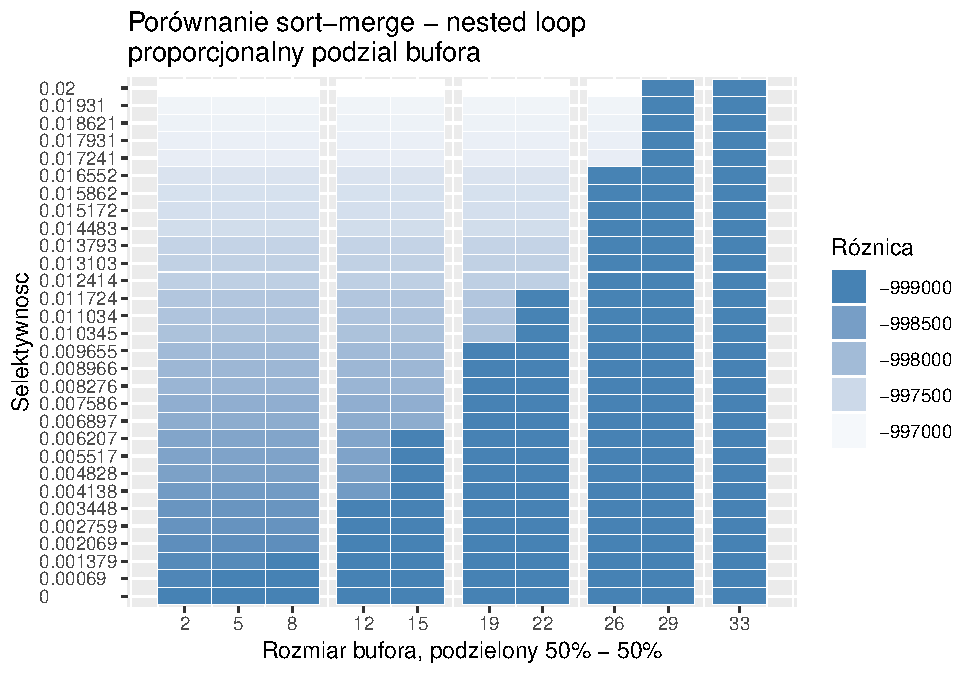
\includegraphics{report_files/figure-latex/plots-1.pdf}
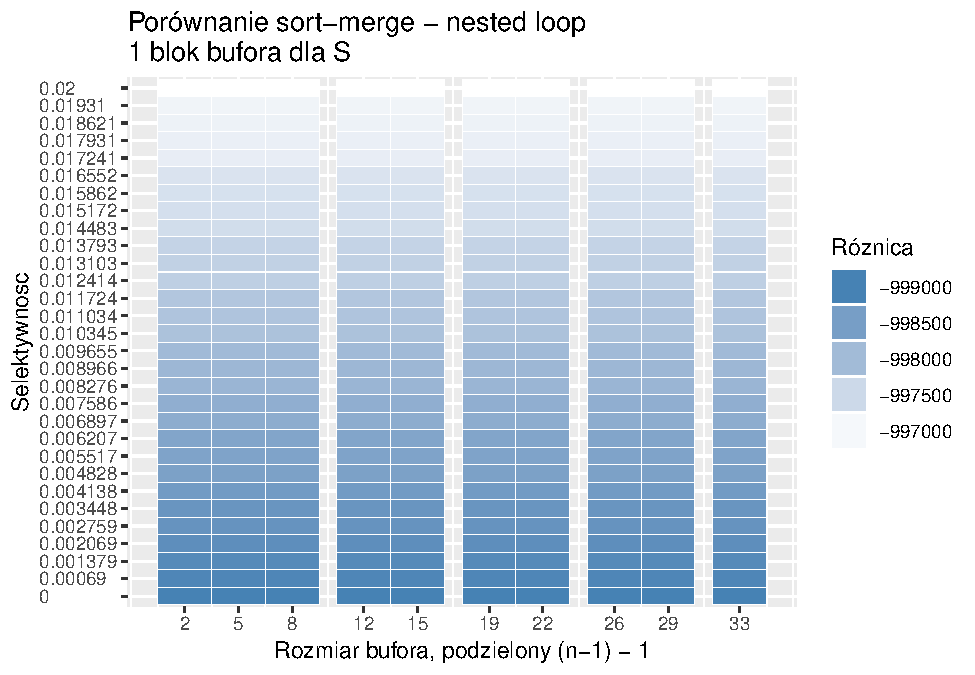
\includegraphics{report_files/figure-latex/plots-2.pdf}
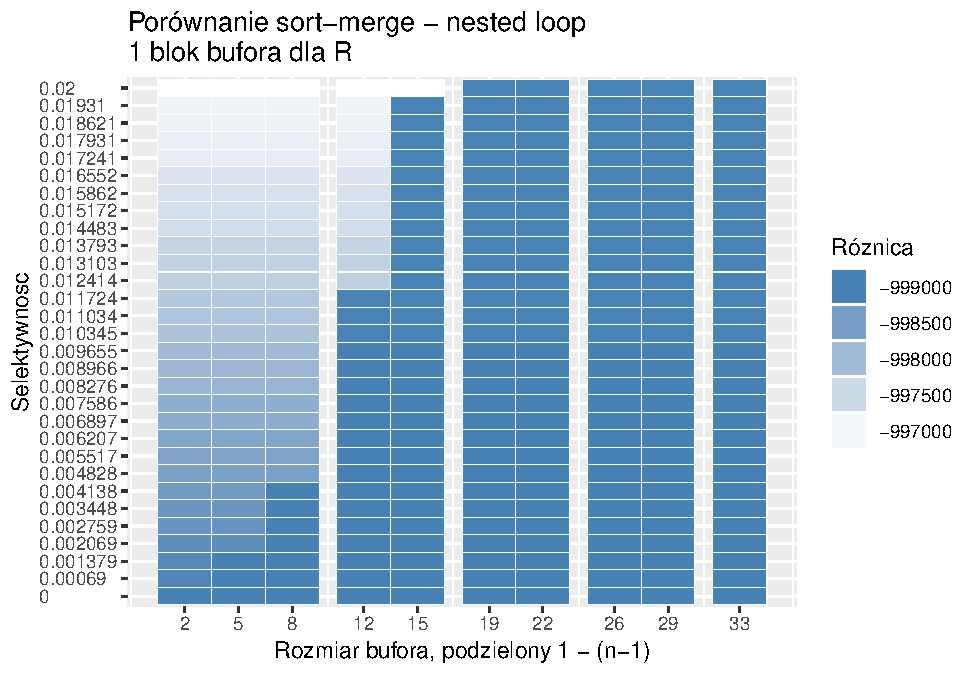
\includegraphics{report_files/figure-latex/plots-3.pdf} \vspace{2mm}

Wykresy przedstawiające wyniki naszych badań jasno prezentują, iż
algortym sort-merge przy badanych przez nas przedziałach współczynnika
selektywności oraz rozmiaru bufora wyraźnie przywyższa wydajnością
algortym nested loop. \vspace{2mm}

Największe różnice pomiędzy algortmami można zauważyć przy podziale
bufora w stosunku 1 - (n-1). W takim przypadku zewnętrznej relacji
biorącej udział w połączeniu przydzielona zostaje większa część bufora.
W takiej sytuacji algorytm nested loop musi wykonać o wiele więcej
dodatkowych iteracji. Różnica ta rośnie dość znacznie wraz ze wzrostem
rozmiaru bufora. \vspace{2mm}

Różnice w wydajności są również widoczne na pierwszym wykresie, kiedy to
bufor jest dzielony w stosunku 50\% - 50\%. W tej sytuacji także można
zauważyć wzrost przewagi wydajności algortymu sort-merge wraz ze
wzrostem rozmiaru bufora, choć przyrost ten jest mniejszy niż w
przypadku opisywanym powyżej. \vspace{2mm}

Najbardziej intersującymn przypadkiem z praktycznego punktu widzenia
jest jednak sytuacja przedstawiona na drugim wykresie. Bufor został w
tym przypadku podzielony w stosunku (n-1) - 1. Jest to sposób podziału
bufora, jaki najczęściej występuje w rzeczywistych sytuacjach przy
wykonywaniu operacji połączenia. Z wykresu dowiadujemy się, iż rozmiaru
bufora w tym przypadku ma niewielki wpływ na różnice w wydajności
działania obu algorytmów. Najistotniejszą zmienną staje się wartość
współczynnika selektywności. Na tym wykresie można zauważyć, iż wraz ze
wzrostem wartości współczynnika selektywności różnice w wydajności
działania obu algorytmów maleją, choć nadal są zdecydowanie zauważalne.
\vspace{2mm}

\section{4 Wnioski}\label{wnioski}

Po przeanalizowaniu wyników eksperymentu narzuca się kilka wniosków. Po
pierwsze, współczynnik selektywności połączenia jest kluczową zmienną,
która decyduje o wydajności algorytmów połączeniowych sort-merge oraz
nested loop. Po drugie, rozmiar bufora nie wpływa na różnicę w
wydajności obu algorytmów przy praktyce najczęściej wykorzystywanym
stosunku podziału bufora ( (n-1) - 1 ). Należy jednak zaznaczyć, że
rozmiar bufora ma, oczywiście, duży wpływ na bezpośrednią wydajność
pojedyńczego algorytmu, chociażby dlatego, iż większy bufor może
oznaczać mniejszą liczbę iteracji algorytmu konieczną do wykonania.
\vspace{2mm}

Otrzymane przez nas wyniki nie były trudne do przewidzenia. Mieliśmy
jednak nadzieję, iż nasze badania pozwolą ustalić bardziej wysublimowaną
tendecję w zmianach różnicy wydajności algortytmów w zależności od
wartości współczynnika selektywności. Tymczasem zależność ta okazała się
być właściwie liniowa. Ciekawsze zależności mogliśmy zaobserwować w
przypadkach, kiedy bufor był dzielony w innych, niż zazwyczaj
wykorzystywane, proporcjach. W takiej sytuacji można zaobserwować
kolejną, w przybliżeniu liniową tendencję wzrostu różnicy w wydajności
algortytmów w zależności od rozmiaru bufora. Ostatecznym wnioskiem z
naszego eksperymentu jest jednak fakt, iż w przypadku operowania na
relacjach, dla których współczynnik selektywności połączenia jest
niewysoki zdecydowanie lepszym wyborem do przeprowadzenia operacji
połączenia relacji ze względu na wydajność jest algorytm sort-merge.
\vspace{2mm}

Istnieje kilka możliwości na rozwinięcie przeprowadzonych przez nas
badań. Jedną z nich jest zwiększenie zakresu analizowanych wartości
współczynnika selektywności. Taka analiza pozwoliłaby stwierdzić czy
istnieją przypadki, ustalonym rozmiarze bufora, w których algorytm
nested loop notuje lepsze wyniki od algorytmu sort-merge oraz, jeśli
takowe występują, pomogłaby sprawdzić jak prezentuje się tendencja zmian
tej różnicy. Oczywiście, współczynnik selektywności jest tylko jedną z
wielu zmiennych jakie można rozpatrywać badając wydajność algorytmów
połączenia dwóch relacji. Dlatego też kolejnym etapem rozwoju naszych
badań mogłoby być bardziej kompleksowe porównanie tych dwóch algorytmów.
Rozpatrzenie większej liczby zmiennych pozwoliłoby na ustalenie większej
liczby szczególnych sytuacji, w których jeden z algorytmów przewyższa
wydajnością drugi. Kolejnym etapem rozwoju mogłoby być dołączenie do
badań większej liczby algorytmów połączeniowych. Na szczególną uwagę
zasługuje rodzina algorytmów haszujących. Taka analiza byłaby jeszcze
bardziej kompletna i umożliwiłaby pełny przegląd sytuacji, w których
powszechnie wykorzystywane w systemach baz danych algorytmy łączenia
relacji są wydajne. \pagebreak

\section{Bibliografia}\label{bibliografia}

\bibliographystyle{abbrv}\bibliography{bibliography}

\hypertarget{refs}{}
\hypertarget{ref-GIT2019}{}
``DB\_SortMergeJoin.'' 2019. {[}online{]} URL:
https://github.com/writ3it/DB\_SortMergeJoin.

\hypertarget{ref-EVA1991}{}
DeWitt, David J., Jeffrey F. Naughton, and Donovan A. Schneider. 1991.
``An Evaluation of Non-Equijoin Algorithms.'' In \emph{Proceedings of
the 17th International Conference on Very Large Data Bases}, 443--52.
VLDB '91. San Francisco, CA, USA: Morgan Kaufmann Publishers Inc.
\url{http://dl.acm.org/citation.cfm?id=645917.672320}.

\hypertarget{ref-SYS2011}{}
Hector Garcia-Molina, Jennifer Widom, Jeffrey D. Ullman. 2011.
\emph{Systemy Baz Danych: Kompletny Podręcznik}. Wydawnictwo Helion.

\hypertarget{ref-PER1989}{}
Schneider, Donovan A., and David J. DeWitt. 1989. ``A Performance
Evaluation of Four Parallel Join Algorithms in a Shared-Nothing
Multiprocessor Environment.'' \emph{SIGMOD Rec.} 18 (2). New York, NY,
USA: ACM: 110--21.
doi:\href{https://doi.org/10.1145/66926.66937}{10.1145/66926.66937}.


\end{document}
